\label{sec:osc-qat-toy}
\begin{figure*}[ht]
     \centering
     \begin{subfigure}[b]{0.324\textwidth}
         \centering
         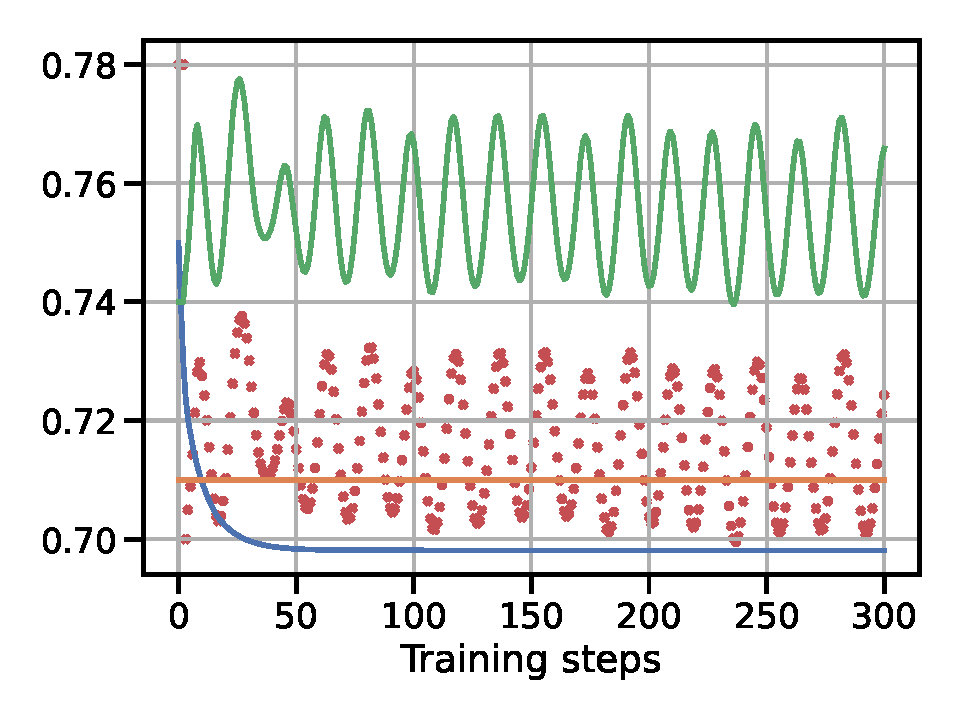
\includegraphics[width=0.99\textwidth]{figures/osc_toy/w_0_train.pdf}
         \caption{}
         \label{fig:toy_w1}
     \end{subfigure}
    %  \hfill
     \begin{subfigure}[b]{0.324\textwidth}
         \centering
         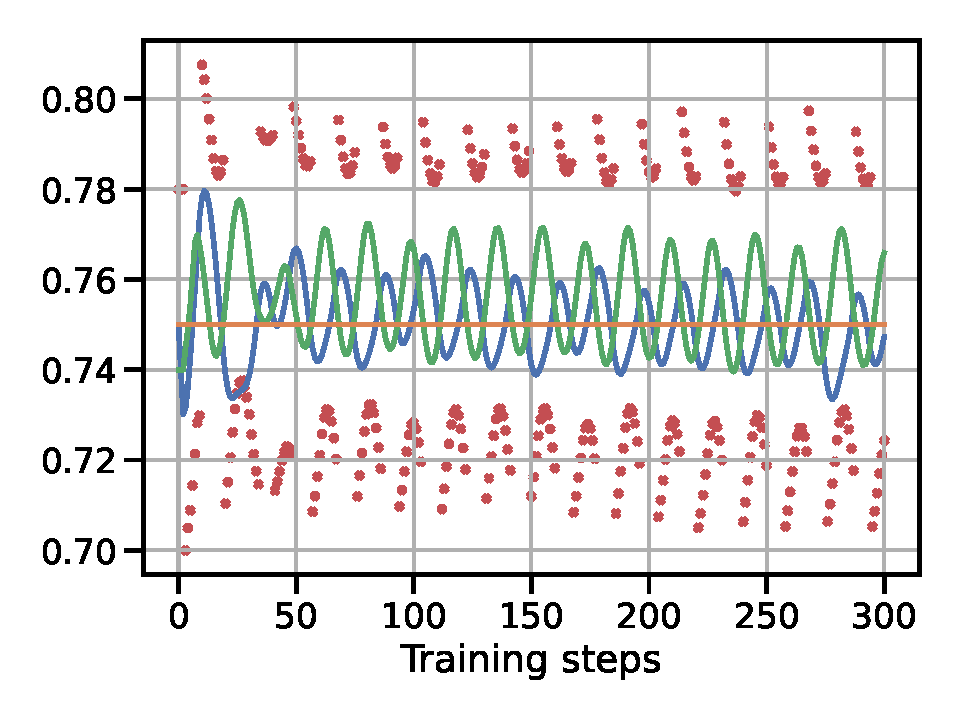
\includegraphics[width=0.99\textwidth]{figures/osc_toy/w_1_train.pdf}
         \caption{}
         \label{fig:toy_w2}
     \end{subfigure}
     \begin{subfigure}[b]{0.324\textwidth}
         \centering
         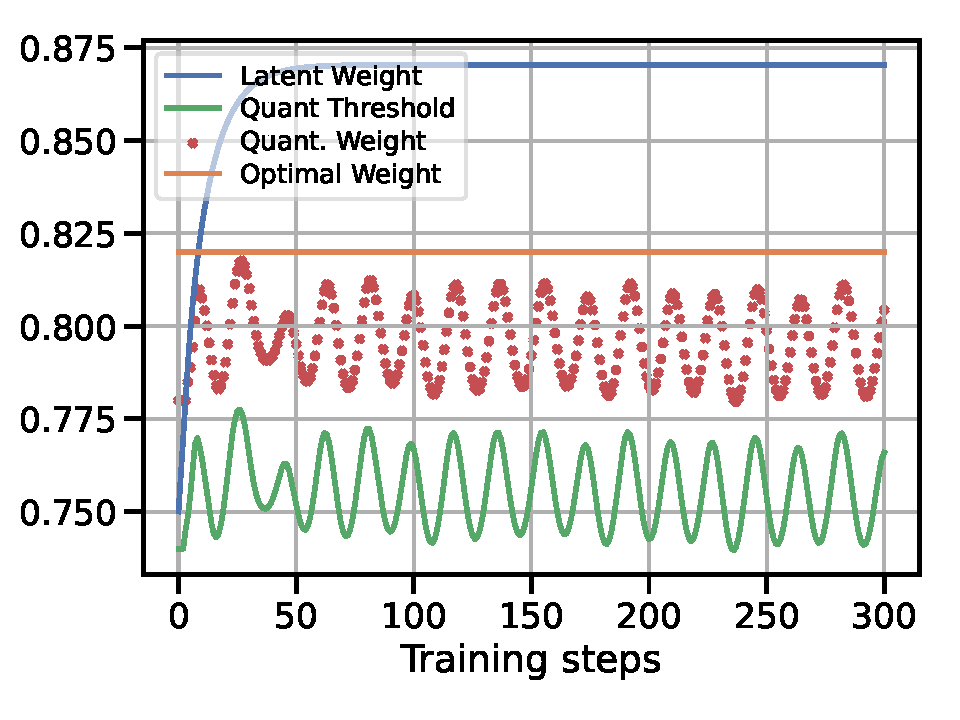
\includegraphics[width=0.99\textwidth]{figures/osc_toy/w_2_train.pdf}
         \caption{}
         \label{fig:toy_w3}
     \end{subfigure}
     % \begin{subfigure}[b]{0.48\textwidth}
     %     \centering
     %     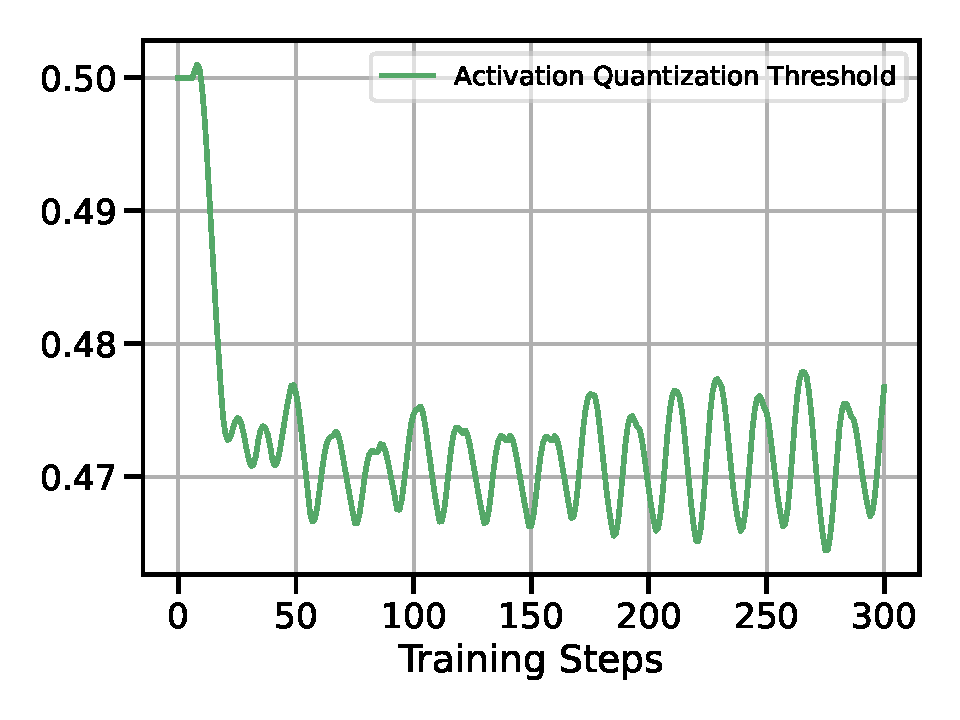
\includegraphics[width=0.99\textwidth]{figures/osc_toy/quant_act_train.pdf}
     %     \caption{}
     %     \label{fig:toy_x}
     % \end{subfigure}
     \vspace{-2ex}
        \caption{\em A toy 3D regression problem to demonstrate the oscillation issue in weight and activation quantization. (a),(b) and (c) Trajectory of different weights during the optimization. Here, it can be seen that oscillation not only affects the latent weights but also the learnable scale factors. Here, "quantization threshold" refers to the quantization boundary in the latent space.} 
        \label{fig:oscillation_toy}
    \vspace{-3ex}
\end{figure*}
\section{Preliminaries}
\label{sec:prelim}
Here we provide a brief background on the quantization-aware training (\acrshort{QAT}) and introduce the issue of oscillations in \acrshort{QAT} using a small toy example.
% \vspace{-2ex}
\begin{figure}
%\begin{figure}
% \vspace{-5ex}
\begin{center}
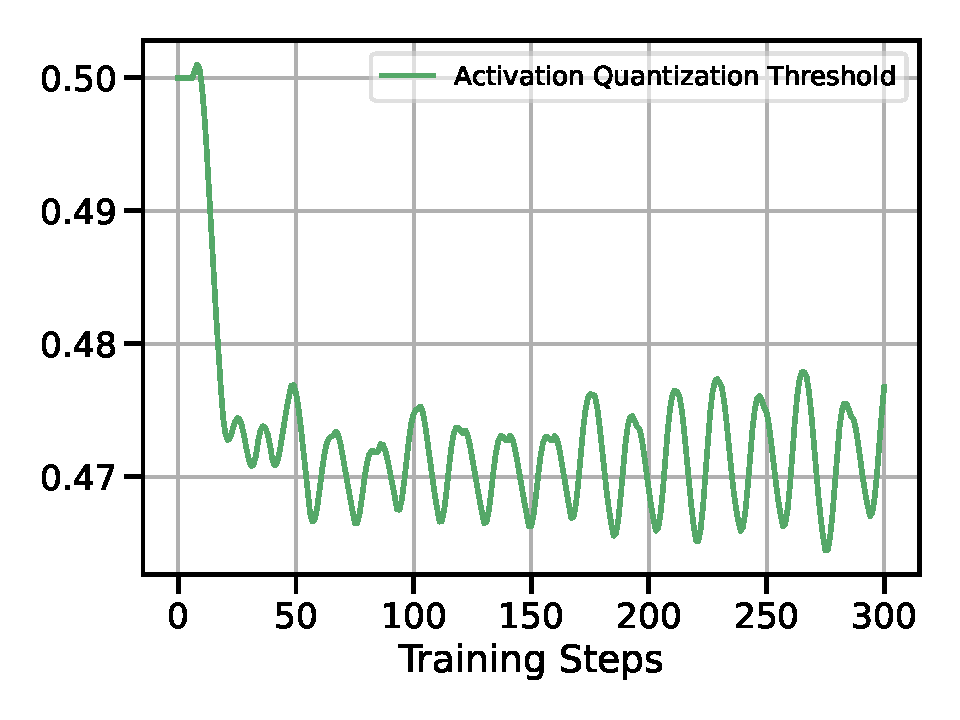
\includegraphics[width=0.70\linewidth]{figures/osc_toy/quant_act_train.pdf}	%trim=[left botm right top]
%\includegraphics[width=\linewidth, trim=1cm 6cm 1cm 1cm, clip=true, page=1]{mda-for-projection.pdf}	%trim=[left botm right top]
\end{center}
\vspace{-4ex}
\caption{\em Trajectory of activation quantization threshold during training for same toy example as in \figref{fig:oscillation_toy}. Even the scale factors for activation quantization oscillate during the optimization.}
 \label{fig:toy_x}
%\end{figure}
\end{figure}
\subsection{Quantization-aware Training 
(\acrshort{QAT})}
\label{sec:prelim-qat}
Quantization-aware training can be achieved by simulating the quantized computational operations during the training of the neural networks. The forward pass of the neural network is encapsulated with a quantization function $q(\cdot)$ that converts full-precision weights and activations into quantized weights and activations. It takes input vector $\vec{w}$ and returns quantized output $\vecq{w}$ given by:
\begin{equation}
    \label{eq:quantization_formulation}
    \vecq{w} = q(\vec{w}; s, u, v) = \ct{s} \cdot \clip{\round*{\frac{\vec{w}}{\ct{s}}}}{\ct{u}}{\ct{v}}, 
\end{equation} 

where $\round*{\cdot}$ is the \textit{round-to-nearest} operator, $\clip{\cdot}{b}{c}$ is a clipping function with lower and upper bounds $b$ and $c$, respectively, $\ct{s}$ is a quantization scale factor. Here, $\ct{u}$ and $\ct{v}$ denote the minimum and maximum range after the quantization. The scale factor $s$ can be learned \cite{lsq, lsq+} during quantization-aware training through backpropagation by approximating the gradient of the rounding operator with \acrshort{STE}. The original full-precision weights $\vec{w}$ are commonly referred to as \textit{latent weights} and gradient descent is performed only on the latent weights for the update. During inference, the quantized weights $\vecq{w}$ are used to compute the convolutional or dense layer output.

Due to the non-differentiability of the quantization function, it is non-trivial to backpropagate through the neural network embedded with such an operation. To this purpose, a commonly used technique for alleviating this issue involves using the straight-through estimator (\acrshort{STE}) \cite{bengio2013estimating, hinton2012ste}. The basic idea of \acrshort{STE} is to approximate the gradient of the rounding operator as 1 within the quantization limits. 

\subsection{Oscillations in \acrshort{QAT}}

\begin{figure*}[ht]
     \centering
     \begin{subfigure}[b]{0.32\textwidth}
         \centering
         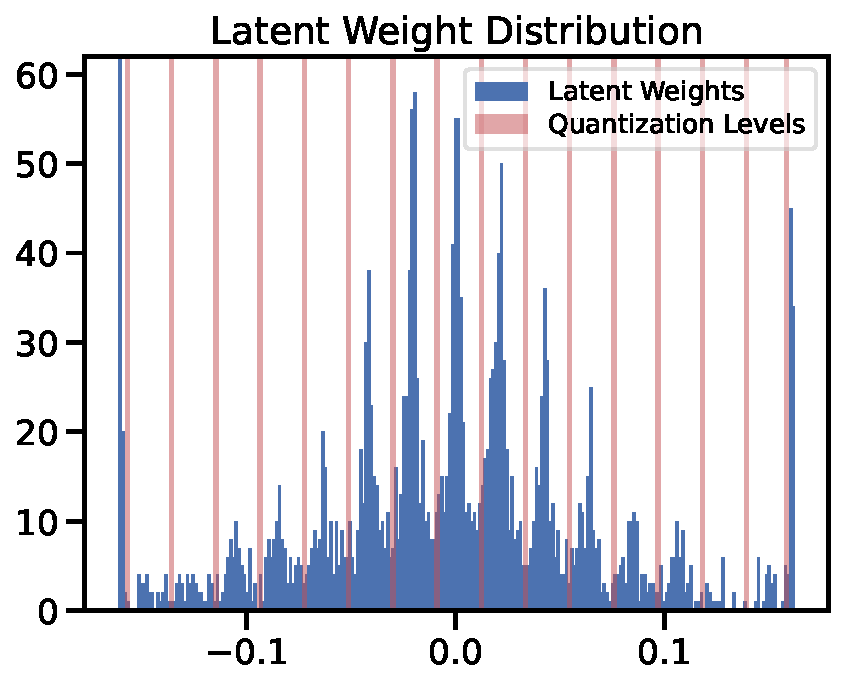
\includegraphics[width=0.99\textwidth]{figures/osc_yolo/4.pdf}
         \caption{}
         \label{fig:latent_yolo}
     \end{subfigure}
    %  \hfill
     \begin{subfigure}[b]{0.33\textwidth}
         \centering
         
\includegraphics[width=1.05\textwidth]{figures/osc_yolo/wts_stepsize.pdf.pdf}
         \caption{}
         \label{fig:scalefactor_wt_yolo}
     \end{subfigure}
     \begin{subfigure}[b]{0.33\textwidth}
         \centering
         
\includegraphics[width=0.99\textwidth]{figures/osc_yolo/acts_stepsize.pdf.pdf}
         \caption{}
         \label{fig:scalefactor_act_yolo}
     \end{subfigure}
    \vspace{-2ex}
        \caption{\em Oscillation issue in \yoloa{}-n variant trained on \coco{} dataset at 4-bit precision using \acrshort{LSQ}~\cite{lsq}. (a) Latent weight distributions of $5^{th}$ convolution layer in \yoloa{}-n, and Scale factors for (b) weight quantization during the last 15K iterations, (c) Scale factors for activation quantization during the last 3K iterations of QAT in YOLOv5-n. Here, it can be clearly observed that latent weights peak exactly at quantization thresholds. Also, both quantization scale factors of weights and activations are not stable even until the end of training.}
        \label{fig:oscillation_yolov5}
    \vspace{-3ex}
\end{figure*}
\label{sec:oscillations}
Recent works~\cite{defossez2022differentiable,nagel2022overcoming} observed the oscillation phenomenon as a side-effect of quantization-aware training with \acrshort{STE} approximation. Due to \acrshort{STE} approximation that passes the gradient through the quantization function, the latent weights oscillate around the quantization threshold.

We illustrate the oscillation phenomenon in \gls{STE} based \acrshort{QAT} using a 3D toy regression problem with both weights and input quantization at 1-bit. Here, we optimize a latent weight vector $\vec{w}$ and scale factors $s_\vec{w}, s_\vec{x}$ for weights and activations respectively with the following objective: 
\begin{equation}
    \argmin_{\vec{w}, s_\vec{w}, s_\vec{x}}\tlossb(\vec{w}, s_\vec{w}, s_\vec{x}) = \eopX{\vec{x}\sim U}{ \|\vec{x}\vec{w}_* - q(\vec{x}, s_\vec{x})q(\vec{w}, s_\vec{w})\|}
    \label{eq:toy_regression_optim}
\end{equation}

Here, $\vec{w}_*$ refers to the optimal ground truth value and $q(\cdot)$ is the quantization function defined in \eqref{eq:quantization_formulation}. We randomly sample data vector $\vec{x}$ from a uniform distribution $U$ within range $[0,1)$. The oscillation behavior during the optimization is shown in \figref{fig:oscillation_toy}. Note that the quantized weights oscillate around the quantization threshold instead of converging close to the optimal value in \figref{fig:toy_w1}, \figref{fig:toy_w2}, and \figref{fig:toy_w3}. Though the underlying reason for oscillation of quantized weights in \figref{fig:toy_w2} is the oscillation of latent weights, oscillation of quantized weights in \figref{fig:toy_w1} and \figref{fig:toy_w3} happens due to oscillation of learnable scale factors. Furthermore, this oscillation behavior is not just restricted to quantized weights but also impacts the quantized activations as can be observed in \figref{fig:toy_x}. In the case of activation quantization, scale factors for activations oscillate as well and this can lead to further performance degradation of quantized models due to sub-optimal minima. Here, we would like to point out that previous work~\cite{nagel2022overcoming} only accounts for the issue of oscillation of latent weights, whereas we show oscillations in learnable scale factors can lead to performance degradation during \acrshort{QAT}.


